\capitulo{5}{Aspectos relevantes del desarrollo del proyecto}



\section{Reproducción del artículo original}

El objetivo de este proyecto es probar nuevos métodos de aprendizaje semi-supervisado aplicados a la detección de ataques. Para lograr este fin, se decidió, en primer lugar, reproducir el artículo original~\cite{zhou2021SemisupervisedRecommendationAttack}, que utiliza el algoritmo \textit{coforest}. Como los autores no especifican detalles de implementación en su artículo (cómo construir perfiles de ataque, dónde encontrar bases de datos o código, etc.), se concluyó que comparar los resultados obtenidos contra los suyos es la mejor forma de determinar la correctitud del trabajo.

\subsection{Experimentación Algoritmos}

\subsubsection{\textit{Co-Forest}}
Para evaluar la calidad del método, se han realizado distintos experimentos con los \textit{dataset} incluídos en la librería \textit{SKlearn} para clasificación. Estos son los mostrados en la tabla~\ref{tabla_datasets_sklearn}. El parámetro $n$ representa el número de instancias que contiene un determinado conjunto de datos, mientras que el parámetro $m$ muestra el número de características que contiene cada una de esas instancias.

\begin{table}
	\small
	\begin{centering}
		
		\begin{tabular}{@{}p{4em} p{20em} r r r @{}}
			\toprule
			\textbf{Nombre} & \textbf{Descripción} & \textbf{Clases} & $n$ & $m$\\ 
			\midrule
			
			Iris & Conjunto de instancias pertenecientes a diferentes tipos de plantas de la especie Iris. & 3 & 150 & 4 \\\\
			Dígitos & Conjunto de instancias que representan una imagen de 8x8 perteneciente a un dígito. & 10 & 1797 & 64 \\\\
			Vino & Conjunto de instancias pertenecientes a tres clases de vino con sus parámetros estimados mediante análisis químico. & 3 & 178 & 13 \\\\
			Cáncer de Mama & Conjunto de instancias que representan parámetros de distintas mujeres que pueden padecer o no cáncer (clasificación binaria). & 2 & 569 & 30 \\
			
			\bottomrule
			
		\end{tabular}
		
	\end{centering}
	\caption{Descripción de los \textit{datasets} utilizados para probar el \textit{co-forest}.}
	\label{tabla_datasets_sklearn}	
\end{table}


Se han realizado diferentes experimentos: algunos relacionados con la fase de entrenamiento y otros con el algoritmo una vez finalizado.

\subsubsection{Fase de entrenamiento}

Como se ha desarrollado en los conceptos teóricos, la fase de entrenamiento en el \textit{co-forest} es iterativa, y finaliza cuando ningún árbol recibe nuevas pseudo-etiquetas que puedan cambiar su comportamiento (en la fase de re-entrenamiento).

Se ha querido estudiar la evolución del \textit{score} (porcentaje de aciertos respecto al total de las predicciones) del algoritmo durante la fase de entrenamiento para los cuatro conjuntos de datos definidos en la tabla~\ref{tabla_datasets_sklearn}. Para ello, se ha realizado una gráfica comprobando cómo evoluciona en función de la iteración en la que se encuentre.

Para garantizar que los resultados obtenidos no son producto de una partición concreta de los datos, se ha realizado validación cruzada (con 10 particiones). Por lo tanto, el porcentaje de datos utilizados para el entrenamiento es el $90\%$ del total (sin estratificación). Los datos de entrenamiento, a su vez, se dividen en etiquetados y no etiquetados. En este caso, el $20\%$ representa los datos etiquetados, y el $80\%$ los no etiquetados, como se puede observar en la imagen~\ref{5_entrenamiento_particiones}. Se han utilizado 20 árboles.

\begin{figure}[h]
	\caption{Gráfica que representa la distribución de los datos.}
	\centering
	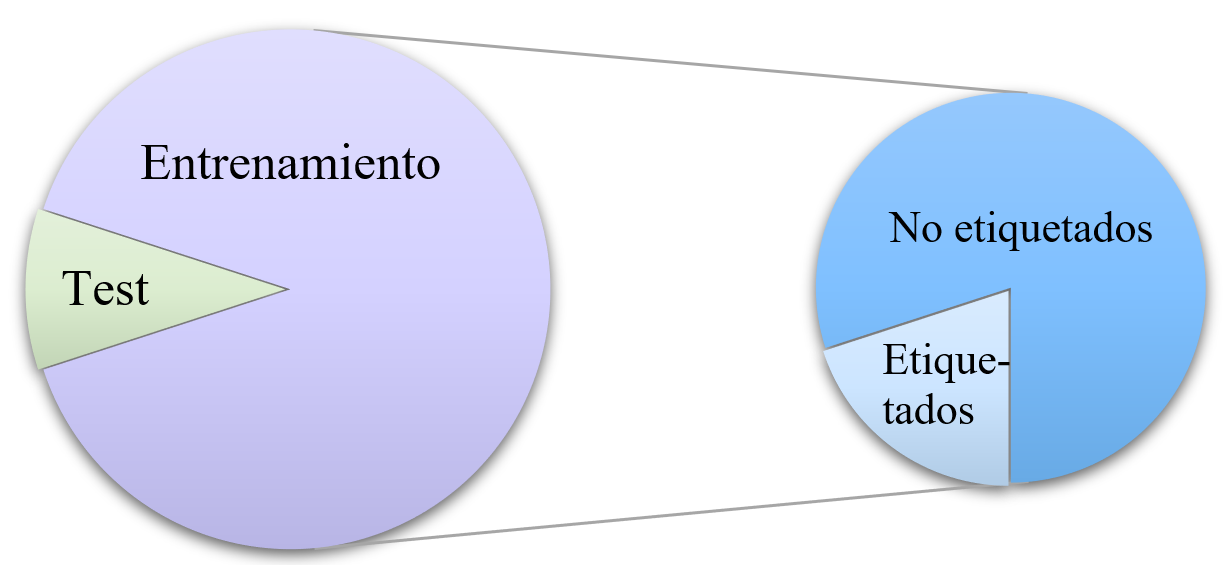
\includegraphics[scale=0.75]{../img/memoria/5_entrenamiento_particiones}
	\label{5_entrenamiento_particiones}
\end{figure}


 La precisión media obtenida se puede ver representada en la gráfica~\ref{5_coforest_score-iteraciones}. Es destacable que, dependiendo de los datos que se utilicen para entrenar el \textit{co-forest}, puede variar el número de iteraciones que se necesiten (incluso dentro de un mismo \textit{dataset}). Por ello, siempre se representa el número máximo de iteraciones realizadas, y para no deformar la media, se ha considerado que el valor de las iteraciones inexistentes es el mismo que el valor obtenido en la última iteración (ya que si, el algoritmo siguiese, el resultado devuelto sería igual debido a que no se re-entrenaría ningún árbol).

\begin{figure}[h]
	\caption{Gráfica que representa el \textit{score} del modelo en función de la iteración en la que se encuentre.}
	\centering
	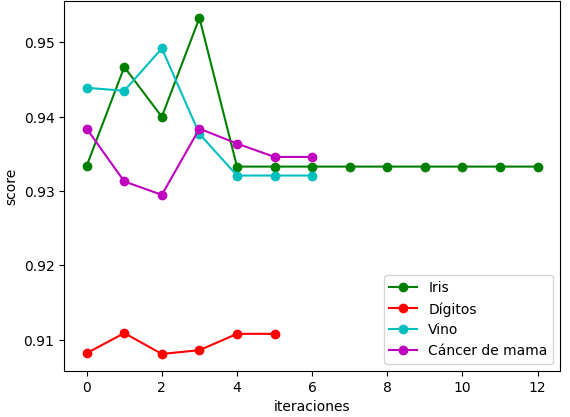
\includegraphics[scale=0.75]{../img/memoria/5_coforest_score-iteraciones}
	\label{5_coforest_score-iteraciones}
\end{figure}

Como se puede comprobar, el modelo mejora los resultados iniciales (exactitud obtenida en la iteración $0$, cuando todavía no se ha realizado entrenamiento semi-supervisado y se cuenta con un \textit{random forest} tradicional) en dos de los conjuntos de datos, mientras que en los otros dos empeora. Este comportamiento es lógico debido a que no todos los modelos son apropiados para todos los conjuntos de datos. 

Si se observa con más detenimiento cada conjunto de datos individualmente (gráfica~\ref{5_coforest_score-iteraciones_individual}), se puede observar que la desviación típica varía considerablemente, por lo que se puede deducir que el modelo podría llegar a ser utilizable en la mayoría de los casos si la partición es la adecuada.

\begin{figure}[h]
	\caption{Gráfica que representa, para cada conjunto de datos, la exactitud media del modelo en función de la iteración en la que se encuentre junto con la desviación estándar para 10 experimentos.}
	\centering
	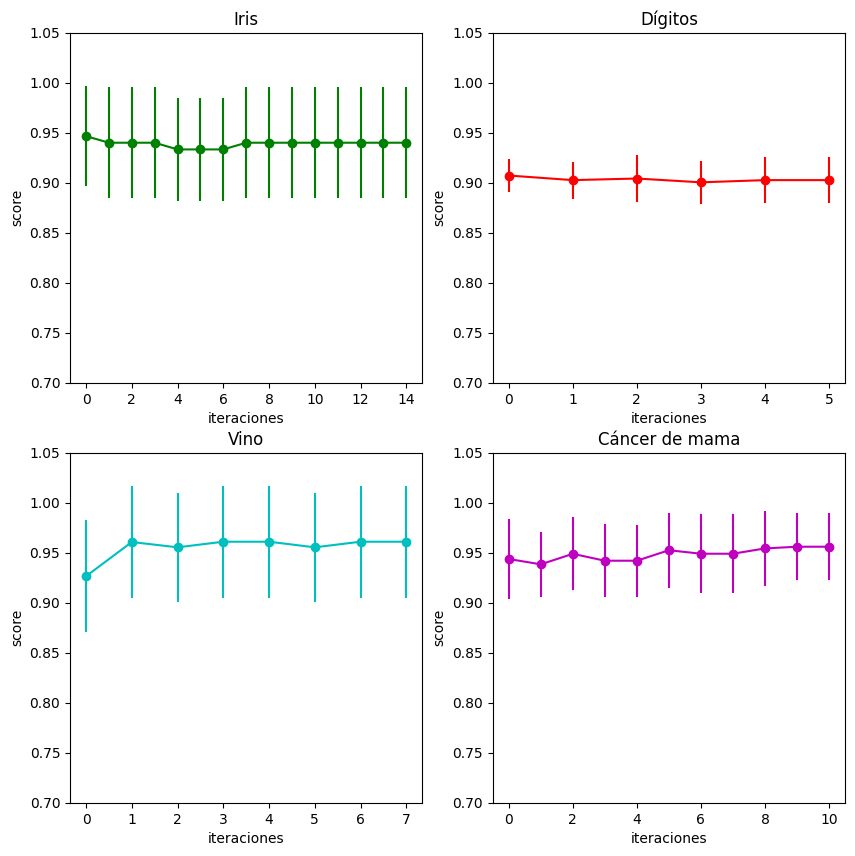
\includegraphics[scale=0.7]{../img/memoria/5_coforest_score-iteraciones_individual}
	\label{5_coforest_score-iteraciones_individual}
\end{figure}


Además, también se ha querido evaluar cómo varía el tiempo de entrenamiento en función del número de instancias utilizadas. Para ello, se ha trabajado con el \textit{dataset} que contiene un mayor número de datos (<<Dígitos>>), y los resultados obtenidos se pueden observar en la gráfica~\ref{5_coforest_tiempo-instancias}. Como se puede comprobar, sigue un crecimiento aproximadamente lineal. La velocidad, en este caso, es alta, pero cabe recordar que depende en gran medida del número de árboles utilizados y de las iteraciones que estos realicen. Se ha representado en la línea negra punteada, además, el resultado del modelo de regresión lineal.

\begin{figure}[h]
	\caption{Gráfica que representa la evolución del tiempo de entrenamiento en función del número de instancias utilizadas.}
	\centering
	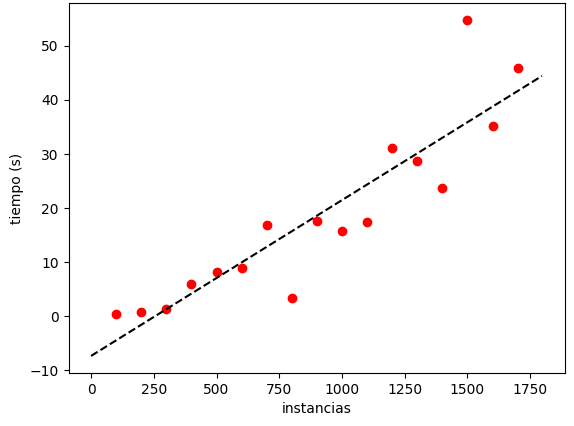
\includegraphics[scale=0.75]{../img/memoria/5_coforest_tiempo-instancias}
	\label{5_coforest_tiempo-instancias}
\end{figure}


\subsubsection{Datos de entrenamiento}

En este apartado de la experimentación, se ha querido evaluar cómo se comporta el \textit{co-forest} en función del porcentaje de datos que se utilice para el entrenamiento. Nuevamente, se han utilizado  $20$ árboles, y la división del conjunto de datos de entrenamiento se ha mantenido: $20\%$ etiquetados y $80\%$ no etiquetados.

Como se puede comprobar en la gráfica~\ref{5_score-porcentaje_entrenamiento}, sigue el comportamiento esperado, y por lo general a más instancias utilizadas para entrenar el modelo, mejor desempeño presenta. Nuevamente, recalcar que el resultado obtenido es la media de 10 experimentos realizados.

\begin{figure}[h]
	\caption{Gráfica que representa la exactitud media del modelo en función del porcentaje de datos (sobre el total de instancias que tiene el \textit{dataset}) utilizados para el entrenamiento.}
	\centering
	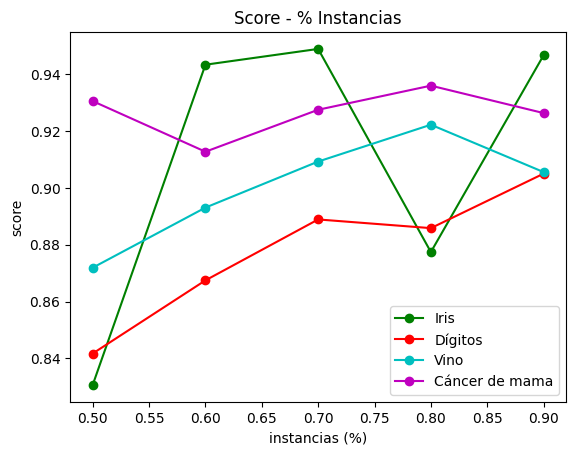
\includegraphics[scale=0.75]{../img/memoria/5_score-porcentaje_entrenamiento}
	\label{5_score-porcentaje_entrenamiento}
\end{figure}

\subsubsection{Número de árboles}

Hasta este momento, todos los resultados han sido realizados para $n=20$. Es decir, utilizando $20$ árboles. Sin embargo, el comportamiento del \textit{co-forest} varía considerablemente en función del número de árboles contenidos en el \textit{ensemble}, lo que motiva la realización del siguiente experimento. Nuevamente, se ha desarrollado utilizando cuatro conjuntos de datos y validación cruzada, por lo que se muestra la media en la exactitud para las $10$ particiones.

Como se puede comprobar en la gráfica~\ref{5_score-arboles}, en general, a más árboles se utilicen, mejor \textit{score} alcanza el \textit{co-forest}. Es destacable que, evidentemente, a mayor $n$, mayor tiempo de procesamiento es requerido. Por lo tanto, se debería alcanzar un compromiso. Por lo general, los autores~\cite{originalCoForest2007} utilizan valores de $n \geq 6$.

\begin{figure}[h]
	\caption{Gráfica que representa la variación del \textit{score} en función del número de árboles del \textit{co-forest}.}
	\centering
	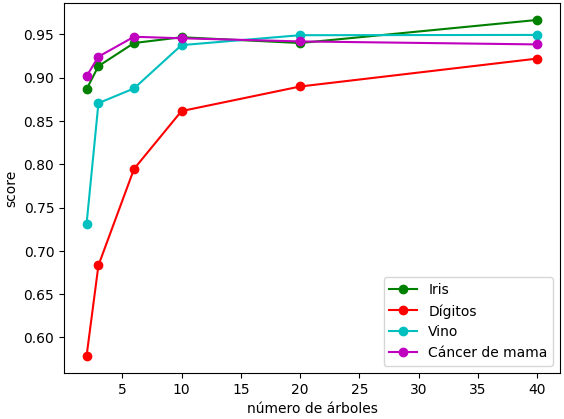
\includegraphics[scale=0.75]{../img/memoria/5_coforest_score-arboles}
	\label{5_score-arboles}
\end{figure}

\subsubsection{Comparativa contra KEEL}

Para asegurar el correcto funcionamiento del algoritmo implementado, se ha decidido comparar contra la herramienta \textit{KEEL}, creada por distintas universidades españolas y financiada por el Ministerio de Educación y Ciencia.

En primer lugar y para tener más capacidad de <<manipulación>>, se optó por descargar los ficheros fuentes de la última versión de GitHub~\cite{keelRepo} en lugar de utilizar la versión compilada que ofrecen los desarrolladores. Se puede consultar cómo en los anexos.

Para comparar los algoritmos en las condiciones más realistas posibles, se definieron las características mostradas en la tabla~\ref{tabla_coforest_keelvsnuestro_diseño}.

\begin{table}
	\begin{centering}
		\begin{tabular}{@{}p{10em} p{20em} @{}}
			\toprule
			\textbf{Parámetro} & \textbf{Valor} \\ 
			\midrule
			$n$ & 6\\
			$\theta$ & 0.75 \\
			\textit{Folds} & 10 \\
			\% etiquetados & 10\% (en el conjunto de entrenamiento). \\
			Comentarios & Para la comparativa se han utilizado los \textit{datasets} <<Iris>> y <<Vino>>. El conjunto <<Iris>> está estratificado (el subconjunto de \textit{test} contiene la misma proporción de clases a probar), mientras que <<Vino>> no lo está. \\
			\bottomrule
			
		\end{tabular}
	\end{centering}
	\caption{Tabla resumen con el diseño del experimento.}
	\label{tabla_coforest_keelvsnuestro_diseño}	
\end{table}

Dentro de los ficheros fuente de KEEL, se pueden encontrar distintos conjuntos de datos con las particiones del \textit{K-cross-validation} ya hechas y que son utilizadas en las ejecuciones de sus experimentos. Para comprobar ambos algoritmos en igualdad de condiciones, se convirtieron dichos archivos \texttt{*.dat} en \texttt{*.csv} y se importaron en la implementación propia mediante la librería Pandas. De esta manera, el único parámetro que no es idéntico entre ambas implementaciones es qué instancias de entre los datos etiquetados seleccionan los árboles para entrenarse en un primer momento (son aleatorios y generar las pequeñas diferencias observadas).

\begin{table}
	\begin{centering}
		
		\begin{tabular}{@{} p{3em} p{6em} p{7em} p{7em} p{7em} @{}}
			\toprule
			\multirow{2}{*}{\textit{ \hfil Fold}} & \multicolumn{2}{c}{\hfil Iris}& \multicolumn{2}{c}{\hfil Vino} \\
			\cmidrule{2-3} \cmidrule{4-5}
			
			& \hfil Propia & \hfil KEEL & \hfil Propia & \hfil KEEL\\ 
			  
			\toprule
			 \hfil 1 &\hfil 1.00	&\hfil 0.87	& \hfil 0.89  & \hfil0.83 \\
			 \hfil 2 &\hfil 0.86	&\hfil 0.80	& \hfil 1.00 	&  \hfil 0.94 \\
			 \hfil 3 & \hfil 1.00	& \hfil 1.00	& \hfil 0.94	& \hfil 1.00 \\
			 \hfil 4 & \hfil 1.00	& \hfil 1.00	& \hfil 0.94	& \hfil 0.89 \\
			 \hfil 5 & \hfil 0.87	& \hfil 1.00	& \hfil 0.65	& \hfil 0.88 \\
			 \hfil 6 & \hfil 0.93	& \hfil 0.93	& \hfil 0.94	& \hfil 0.71 \\
			 \hfil 7 & \hfil 0.93	& \hfil 1.00	& \hfil 0.83	& \hfil 0.89 \\
			 \hfil 8 & \hfil 0.93	& \hfil 0.93	& \hfil 0.94	& \hfil 0.78 \\
		 	 \hfil 	9 & \hfil 0.93	& \hfil 0.93	& \hfil 0.67	& \hfil 0.72 \\
			 \hfil 10& \hfil 0.87	& \hfil 0.87	& \hfil 0.94	& \hfil 0.94 \\
			 \midrule
			 \hfil Media 			& \hfil 0.93	& \hfil 0.93	& \hfil 0.88	& \hfil 0.86 \\
			\bottomrule
		\end{tabular}
	\end{centering}

	\caption{Comparativa entre la exactitud del \textit{co-forest} de KEEL y el propio sobre el conjunto de \textit{test}.}
	\label{tabla_coforest_keelvsnuestro}	
\end{table}

Los resultados obtenidos se pueden observar en la tabla~\ref{tabla_coforest_keelvsnuestro}. Como se puede comprobar, ambos algoritmos obtienen resultados prácticamente idénticos, siendo un poco superior el porcentaje de acierto logrado por la herramienta implementada propia en el caso del \textit{dataset} <<Vino>>.


\subsection{Detección de ataques}

En el \textit{paper} original~\cite{zhou2021SemisupervisedRecommendationAttack} se utilizan tes conjuntos de datos para probar la efectividad del \textit{co-forest}: MovieLens10M, MovieLens25M y Amazon.

\subsubsection{MovieLens 10M: Descripción}
 
MovieLens10M~\cite{groupLensDatasets} es un conjunto de datos utilizado típicamente en la investigación y desarrollo de sistemas de recomendación. Contiene 10\,000\,054 opiniones generadas por 71\,567 usuarios acerca de 10\,681 películas. Estas reseñas han sido recopiladas del servicio \textit{online} de películas MovieLens\footnote{https://movielens.org/}.

Los usuarios han sido seleccionados aleatoriamente entre los perfiles que tengan más de 20 películas valoradas y está documentado que todos son auténticos~\cite{zhou2021SemisupervisedRecommendationAttack} y pertenecen a usuarios reales. Por lo tanto, los perfiles atacantes han de ser construidos mediante programación.

\subsubsection{MovieLens 10M: Generación de vectores de características.}

Como se puede comprobar en el \textit{paper} de Zhou y Duan~\cite{zhou2021SemisupervisedRecommendationAttack} los perfiles de usuarios normales son distinguibles de los atacantes debido a su forma de puntuar. En función de estos hábitos, se puede elaborar un método de detección basado en ventanas.

En primer lugar, se dividen todos los ítems del \textit{dataset} en ventanas, consiguiendo un conjunto de $J$ ventanas (\{$w_1, w_2, ..., w_J$\}). No se aplica ningún orden especial, sino que se respeta el que aparece en la propia base de datos. El número de ítems que posee cada ventana se reparte como se muestra en la ecuación~\ref{eqn:window_reparto}, donde $Q$ es el cociente de dividir el número total de ítems entre $J$.
	
\[|w_j| = \left\{ \begin{array}{lr} Q + 1, & j < q\\ Q, & j \ge q \label{eqn:window_reparto} \end{array} \right. \] 

Posteriormente se calcula, para cada usuario y ventana, $NRW_{u, w_j}$ y  $WNRW_{u, w_j}$ como se muestra en las ecuaciones~\ref{eqn:NRW} y \ref{eqn:WNRW} respectivamente. $NRW$ son las siglas de \textit{number of ratings per window}, y $WNRW$ \textit{weighted number of ratings per window}. Es decir, para un determinado usuario, el número de votaciones que haya realizado en una ventana y el ratio de esta respecto al total.

\begin{equation}\label{eqn:NRW} NRW_{u, w_j} = \sum_{i\in w_j, r_{u,i} \ne 0}^{} 1 \end{equation}
\begin{equation}\label{eqn:WNRW} WNRW_{u, w_j} = \frac{\sum_{i\in w_j, r_{u,i} \ne 0}^{} 1}{\sum_{i\in I, r_{u,i} \ne 0}^{} 1} \end{equation}

Aplicando estas fórmulas como se muestra en el pseudocódigo~\ref{alg:window_feature_extraction}, se obtienen los vectores de características. Como se puede deducir, este algoritmo se aplica equitativamente a perfiles genuinos y atacantes, ya que únicamente se precisan las reseñas del usuario. Para una mayor comodidad a la hora de experimentar con estos datos, se han generado ficheros \texttt{.csv} con los vectores de características que posteriormente se importarán mediante Pandas para generar conjuntos de entrenamiento y \textit{test}. Debido a que se trata de un problema de clasificación binaria, los perfiles atacantes reciben una etiqueta de $1$ y los verdaderos un $0$. Cabe destacar, que debido a que en el conjunto de MovieLens todos los usuarios son genuinos, se han de generar las reseñas de los perfiles atacantes. 

\begin{algorithm}
	\KwIn{Conjunto de usuarios $S$, número de ventanas $J$, conjunto de reseñas del usuario $R$.}
	\KwOut{Conjunto de vectores de características $X$.}
	\BlankLine
	$X \leftarrow \emptyset$\\
	\For{$u \in S$}{
		\For{$j \in J$}{
			Calcular $NRW_{u, w_j}$\\
			Calcular $WNRW_{u, w_j}$\\
		}
		$x_u \leftarrow \{NRW_{u, w_1},  WNRW_{u, w_1},  ..., NRW_{u, w_j},  WNRW_{u, w_j}\}$\\
		$X \leftarrow X \cup x_u$\\
	}
	\Return{$X$}
	\caption{Algoritmo de generación de vectores de características.}
	\label{alg:window_feature_extraction}
\end{algorithm}


\subsubsection{MovieLens 10M: Creación de reseñas atacantes}

Se ha incluido tres tipos de ataques distintos: \textit{random}, \textit{average} y \textit{bandwagon}. En primer lugar, se han sintetizado las reseñas y posteriormente se han generado los vectores de características idénticamente a los perfiles verdaderos.

La metodología de construcción de las valoraciones sigue los modelos estadísticos expuestos en la sección teórica del proyecto. Sin embargo, se puede visualizar un resumen de los escogidos en la tabla~\ref{ataques_coforest}.

\begin{table}
\begin{centering}
	
	\begin{tabular}{@{}p{5em} p{5em} p{11em} p{9em}@{}}
		\toprule
		\textbf{Modelo} & $\mathbf{I_S}$ & \textbf{Valoración} $\mathbf{I_F}$ &  \textbf{Valoración} $\mathbf{I_t}$\\ 
		\midrule
		Random & $\emptyset$ & Aleatoria siguiendo una distribución $\mathcal{N}(\mu,\,\sigma)$. & máxima o mínima \\
		Average & $\emptyset$ & Aleatoria siguiendo una distribución $\mathcal{N}(\mu_i,\,\sigma_i)$. & máxima o mínima\\
		Bandwagon (random) & $k$ ítems más populares & Aleatoria siguiendo una distribución $\mathcal{N}(\mu,\,\sigma)$. & máxima o mínima\\
		\bottomrule
	\end{tabular}
	\caption{Características estadísticas de los tipos de perfiles atacantes.}
	\label{ataques_coforest}	

\end{centering}
\end{table}

Para construir las reseñas pertenecientes a un ataque del tipo \textit{random}, se ha obtenido, en primer lugar, la media de la puntuación general para todas las películas del sistema y su desviación. Los ítems de relleno han sido seleccionados aleatoriamente entre toda la base de datos (excluyendo, evidentemente, los ítems objetivo), y se ha asignado a cada uno una puntuación aleatoria siguiendo una distribución normal parametrizada por la media y desviación <<global>> del sistema. Evidentemente, esta puntuación ha sido corregida para que se encuentre entre los rangos admitidos (por ejemplo, de $0$ a $5$ estrellas). Debido a que el método de detección utilizado no necesita fechas, el campo perteneciente a la \textit{timestamp} no ha sido rellenado. Posteriormente, se ha asignado la máxima puntuación a los ítems objetivo (\textit{push attack}).

En el caso del ataque \textit{average}, el procedimiento ha sido el mismo, solo que en este caso las puntuaciones de los ítems de relleno son más representativas. En lugar de seguir una normal parametrizada por las características del sistema a nivel global, se ha calculado para cada película su media y su desviación, y se ha asignado una valoración aleatoria que sigue esta distribución. Es decir, cada ítem de relleno recibe una puntuación aleatoria que sigue una distribución normal con media la correspondiente a ese ítem en concreto, y con su respectiva desviación. En caso de que se escoja una película nunca antes valorada, la media utilizada es la media del rango (por ejemplo, $2.5$ estrellas) y la desviación es $0$.

Por último, el ataque \textit{bandwagon}. Este ataque se realiza exactamente igual que el \textit{random} solo que, además, se añade un conjunto nuevo, los <<ítems seleccionados>> o $I_s$. En este caso, se escogen los $k$ ítems más populares de la base de datos (se entiende por más <<popular>> aquel ítem que posea más valoraciones). Evidentemente, este conjunto se excluye (además de los ítems objetivo) a la hora de escoger los ítems de relleno. La valoración asignada a $I_s$ ha sido o bien la máxima, o bien la mínima (en función de su nota media).














